\documentclass[11pt]{report}
\usepackage{setspace}
\usepackage{cite}
\usepackage{amsmath}
\usepackage{graphicx}
\usepackage{verbatim}
\usepackage{listings}
\usepackage{mathbbol}
\newcommand{\argmax}{\arg\!\max}

\doublespacing
\title{Working Title}
\author{Dale Markowitz}
\begin{document}

\maketitle{}

\begin{abstract}
Sustaining one’s attention is a perpetually difficult tasks for humans, not only because our minds tend to wander but also because we lose attention unpredictably, often not noticing our own attentional lapses until long after they have begun.  In this experiment, we explore how EEG-derived neurofeedback provided to participants in real-time can help humans to notice not only to notice when they have lost attention, but also create better mental representations of the task at hand.  Participants responded to a task in which they were instructed to attend to pictures of faces and ignore superimposed pictures of places, or attend to pictures of places and ignore faces, while receiving real-time neurofeedback from a wireless EEG headset.  We provided participants neurofeedback derived from how “face-like” or “place-like” their EEG data appeared when categorized by a classifier.  We found that the “classifiability” of each participant’s EEG data predicted how will he/she performed on a face/place task without feedback, and that later providing participants with neurofeedback was correlated with both higher task accuracy post-feedback as well as higher classifiability post-feedback.	
\end{abstract}

\section{Introduction}
It’s a classic experiment: balance on one foot with your eyes opened, and then balance on one foot with your eyes closed.  The first is easy, the second is impossible.  Why?  Because our brains are experts in control theory.  In the first case, we stand on one foot starting with our best guess of the correct posture and position we should take to maintain balance.  Meanwhile, our eyes observe how closely our actual position matches our intended position, and dictates to our bodies how to adjust our stances to bring ourselves closer to balance.  When we close our eyes, we remove a channel of immediate feedback on how our actions effect our balance, and hence balancing becomes all the more challenging.
Feedback is clearly important in helping us successfully achieve our goals—both the literal, immediate feedback we use in tasks like balancing and the more subtle type of feedback we might look for from a final exam grade or from a midyear review.  But what if we could use feedback to help ourselves improves the most fundamental determiner of our actions—-our thoughts?  In this thesis, we explore how humans can learn to improve their attention by receiving real-time feedback on their internal attentional states.  We use an inexpensive and nonintrusive EEG device to measure the fluctuating voltages along participants’ scalps, and interpret this data using machine learning techniques to construct a metric of participants’ attention.  We then provide participants real-time feedback on how well they are attending to their given tasks by making the tasks harder or easier if the participants’ are attending weakly or strongly, respectively.  Brain-Computer Interfaces (BCI’s) for attention training are not new—in fact, they have lived a rich life as a therapy for ADHD of undetermined efficacy—but we believe that our use of machine learning techniques to give participants feedback determined directly by the contents of their thoughts can make attention training much more effective than before. 

\section{Background}

Neurofeedback was first shown to be effective when, in 1985, Joe Kamiya at the University of Chicago taught an adult to alter his brain-wave frequencies\cite{Lofthouse}. {\bf TBD}

\subsection{Machine Learning for EEG/fMRI Data}
Traditional fMRI and EEG analyses have focused on understanding the relationships between spatial brain regions or voltage frequencies and function.  On the other hand, machine learning techniques that have been highly fruitful in domains including object, handwriting, and speech recognition system, discover relationships between input data and its categories by fitting a model from a given model class to data in a way that minimizes the error of that model on the data.  As a result, machine learning techniques can find representations and mappings of large, high-dimensional data sets that are more subtle than what a human being could predict by examining the data through traditional techniques alone.  The application of machine learning techniques to fMRI data—often called multi-voxel pattern analysis or MVPA—has thus been highly fruitful\cite{Norman}.  For example, Kamitani et al. \cite{Kamitani} used MVPA to understand how line orientation is represented in the visual cortex, a phenomenon which occurs at cortical columns at the sub-voxel scale.   Using MVPA (particularly support vector machines), they were able to recognize brain activity associated with orientation of gratings, even though this phenomenon occurs beyond the resolution of fMRI, by taking advantage of the patterns of voxel activation spread throughout the visual cortex.  
Machine learning techniques have also proved useful for EEG data analysis.  Several studies use support vector machines to map EEG signals to prosthetic control (See Ken’s paper citation 6,7,8,9,10,11).  {\bf TBD}

\subsection{Real-Time EEG BCI's}
Research in EEG-based BCI's is very active, particularly in the domain of assistive technology.  It is a prime candidate for assisting sufferers of motor paralysis, because it is not only inexpensive but also nonintrusive compared to, say, electrocortiography-based (ECoG) BCI's in which electrodes are placed directly on the surface of a patient's brain.  For example, the Thought-Translational Device (TTD)\cite{Birbaumer} was an EEG-based BCI that allowed ALS patients to select letters from a screen by modulating Slow Cortical Potentials (SCPs).  Patients learned to modulate SCPs via operant conditioning provided by the TTD system, training over the course of six months to six years.  On average, the participants were able to communicate with a speed of about one word per minute.  

\subsection{EEG Signals and Attention}
Many studies have found evidence that oscillation frequencies of EEG voltages relate to attention.  Ray et al\cite{Ray} studied EEG signals that reflect attention to internal and external tasks (recognizing faces versus mental arithmetic, for example), and found that alpha activity was greater in the internal versus external attentional tasks.   {\bf TBD} 

\subsection{Attention Training}
	EEG neurofeedback training for sustained attention has been of particular interest in serving as a treatment for ADHD.  A 2012 review\cite{Lofthouse} of 14 such treatments found that the feedback was ``probably efficacious'' but found that most experiments suffered from design flaws.  Most studies examined theta/beta frequencies with a single electrode placed at Cz according to the 10-20 electrode system, and gave participants neurofeedback through a video game.  The theoretical motivation for such analyses comes from the fact that many patients with ADHD have shown stronger power in the theta and slow-wave frequencies than controls, and less beta power in the central and frontal regions.  Indeed, several studies\cite{Barry} have found that EEG analyses of these frequency ranges can predict the presence of ADHD in patients with accuracies above 85\%.  A limitation of such vigilance-based attention analyses is that it does not distinguish between a participant being focused in general, and being focused on a target task at hand. {\bf TBD}

\section{Contributions}
Our experiment is inspired largely by deBettencourt et al.\cite{deBettencourt}, who conducted a similar study using fMRI rather than EEG data.  In both experiments, participants receive feedback related to how confidently a given classifier classifies the participant’s fMRI or EEG data as being focused on the target category.  Past attentional training experiments have used alpha power as a metric for attention, but we find this approach problematic because the feedback relates only to general “vigilance,” and has no knowledge of to what subject a participant’s vigilance is attending.  Our feedback, on the other hind, is directly tied to the content of a participant’s thoughts.

\section{Experiment Setup}

\subsection{Definitions}
\begin{table}[h]
\begin{tabular}{p{4cm}|p{10cm}}
\textbf{Trial}  & a 50 second long interval in which a single face/place pair is displayed to the participant  \\
\\
\textbf{Non-Lure Trial} & a “go” trial, in which the correct response for the participant is to respond (i.e. click).  These trials make up 90 percent of all trials.\\
\\
\textbf{Lure Trial}  & a “no-go” trial in which the correct response is not to respond (no click).  These trials make up 10 percent of all trials.\\
\\
\textbf{Block} & a set of 50 trials during which participants are instructed to attend to only faces or to only places\\
\\
\textbf{Pre-Training Block}  & a block in which the participant is not wearing the Emotiv.  Data is collected to evaluate prior participant performance on the face/place task. \\
\\
\textbf{Stable Block} & a block in which the participant is wearing the Emotiv, but not receiving neurofeedback.  Data collected during this time period is used to create a model for later EEG classification.\\
\\
\textbf{Feedback Block} & a block in which the participant receives real-time feedback classified by the model created with data from the stable blocks.
\end{tabular}
\end{table}

\subsection{Setup}
In this experiment, participants were shown superimposed pictures of faces and places.  They were then instructed to either focus on images of faces and ignore images of places, or ignore faces and focus on  places.  When focusing on faces, participants were asked to click a button if a shown face was female, and to not click if a shown face is male (which particular gender a participant was asked to respond to is randomized).  Similarly, participants were asked to click a button during a place task if the shown image was outdoors (indoors), and restrain from clicking with then place was indoors (outdoors).  Each superimposed picture was shown to the participant for 50 seconds during a trial.  During both tasks, 90 percent of images shown to participants were from the click or “go” category, and the remaining 10 percent were from the no click or “no-go” category.  As a result of the infrequency of the no-go trials, these trials were much more difficult to respond to correctly than the go trials. Thus we call these no-go trials {\bf lure} trials, since they “lure” a participant to continue clicking after having clicked through a string of go trials.  

During the first 30 minutes of the experiment, participants were shown 50/50 mixtures of faces and places.  Data collected from this time period was then used to create a model that, given a reading of an EEG measurement, predicted the probability of that data point belonging to the “face” or “place” category (i.e. was this data point more likely collected when the participant was participating in a face task, or a place task?).  During the remaining 20 minutes of the experiment, the image mixture ratio--the percent of face to place in the superimposed image stimulus--was determined by how ``face=like'' or ``place-like'' the classifier rated participants' brains.  When a participant was supposed to be focusing on the face task but their brain looked ``face-y'', the face was made more difficult to see, so that the task become more challenging.  Conversely, when the classifier predicted with high confidence that the participant's brain resembled the target class category, the image ratio was altered so that the task became easier.

\section{Neuromancer Software/Hardware Stack}

In order to run the aforementioned experiment, the author created a software stack to coordinate data collection from the EEG headset along with showing participants stimuli, collection participant responses, and analyzing the collected data in real time.  The EEG headset chosen for this experiment was the Epoch Emotiv, as described below.  The software framework for coordinating the experiment, Nueromancer, was built in many languages and consists of many interchangeable modules, also described below.

\subsection{Epoch Emotiv}
	\begin{figure}[t]
	
	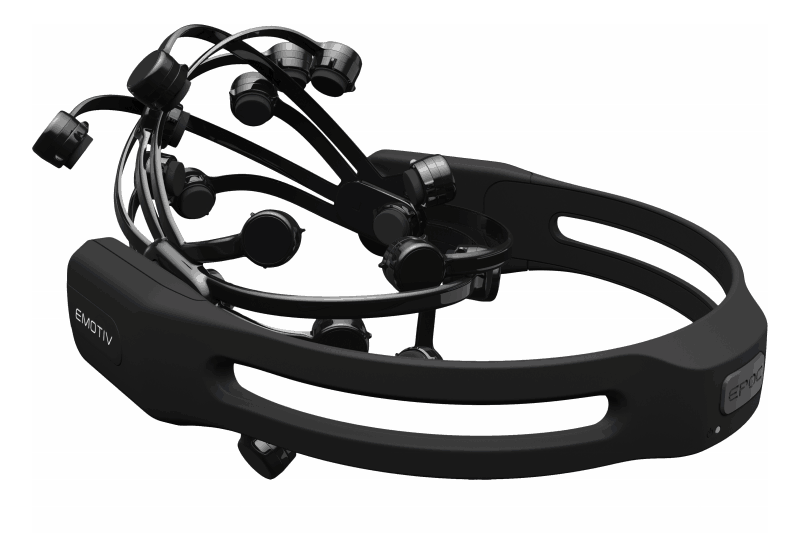
\includegraphics[width=12cm]{emotiv}	
	\centering
	\caption{Epoch Emotiv Headset. https://emotiv.com/media/}
	\end{figure}
	
	The Epoch Emotiv\cite{emotiv} is a wireless, hundred-dollar, consumer-grade EEG headset.  It contains fourteen data channels plus two reference channels, sampling at 128 samples per second.  The headset communicates with a computer via a proprietary Bluetooth dongle.
	
	The Emotiv is extremely susceptible to motion/eyeblink artifacts, and thus a research-grade EEG device with (for example) 32 or 64 electrodes may be preferable in many experiment settings.  However, whereas a typical EEG setup might use an electrode cap which connects electrodes to participants' scalps via messy conductive gel, the Emotiv can be cleanly placed on participants' heads using only sponges soaked in conductive solution (contact solution, for example).  Thus the Emotiv often can be setup more quickly than a typical EEG.  However, the headset design comes at the cost off being difficult to align consistently across participants heads, as well as being unable to penetrate thick hair.  At least four participants were unable to complete this experiment because the of these reasons.
	
	At least a handful of psychology experiments have used the Emotiv, including several from Princeton Senior Theses (\cite{Rafidi}, \cite{Adelson}, and of course this thesis)!  Additionally, Duvinage et al.\cite{Duvinage} explored the performance of the Emotiv for classifying P300 signals, an event-related potential that occurs roughly 300 milliseconds after a participant sees an ``oddball'' stimulus in a sequence of stimuli\cite{p300}.  Duvinage found that the Emotiv performs significantly worse than a medical grade EEG device, and recommend its use only in situations in which reliability and a high signal-to-noise ratio are non-critical.
	
\subsection{Neuromancer Overview}
\begin{figure*}
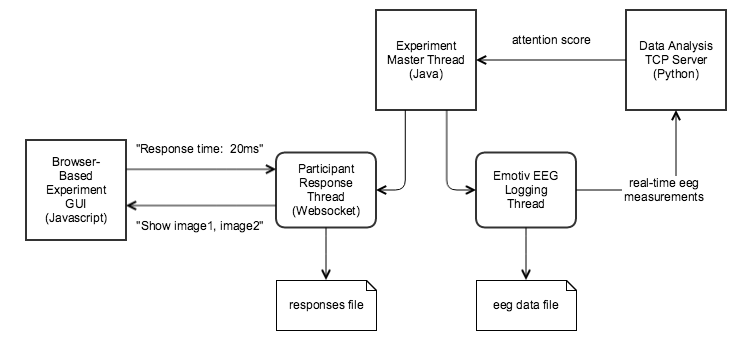
\includegraphics[width=12cm]{neuromancer_anatomy}
\caption{Neuromancer Component Diagram}
\end{figure*}

The Neuromancer software stack consists of three parts: the experiment GUI, data analysis server, and experiment controller.  The experiment GUI displays images to the participant and records participant responses.  The data analysis server analyzes collected data, creates a model, and classifies data used for real-time feedback.  The experiment controller coordinates collecting EEG data, controlling the experiment GUI, and writing responses and metadata to file.

\subsection{Experiment Controller}
The Neuromancer experiment controller was written as Java (so chosen because the Emotiv API was available in Java).  At its start, the controller creates a thread dedicated to polling the Emotiv for data.  It continually writes this data to file using a buffered writing structure.  This logging thread exposes methods to the main controller thread for starting, pausing, and stopping data collection.  The logging thread starts logging when the participant is shown the first block of the experiment, and stopped when the experiment ends.
  
In addition to running data collection in the background, the experiment controller coordinates the evolution of the experiment through its phases. That is, the controller guides the experiment's transition from pre-training to stable to feedback to post-training phase, as well as the transition from block to block and trial to trial.   

The design of the experiment controller, which is the core of the Neuromancer software stack, was built with as a compromise between flexibility and practicality.  At its core, it conducts the experiment via a DFA inner class as explained below.  Future users wishing to modify Neuromancer for their own experiments can do so by modifying this DFA inner class.  

A DFA or deterministic finite automaton is a deterministic finite state machine.  It consists of a series of states and a set of rules for transitioning between states.  An diagram of the DFA designed for this experiment is given below:

\lstset{language=Java, basicstyle={\singlespacing}, caption=Dfa Class, breaklines=true}
\begin{lstlisting}
	private class Dfa{
		public void start(){
			/* Method to start DFA, may include setting initial state, displaying start message, etc. */
			return;
		}
		
		public void doNext(boolean fromTimer){
			/* Describes how the DFA transitions from its current state to the next state.  The boolean parameter fromTimer is given so that this can be triggered either by a timer, or (for example) via a user-initiated event (like a mouse click).
			*/
			return;
		}
		
		
	}
\end{lstlisting}

\subsection{Graphical User Interface}
	The user interface in this experiment was built to run in a web browser, which is in this case Google Chrome.  Writing a browser-based experiment interface yields many potential advantages over more specialized, language-specific GUI frameworks.  For one, many templates exist both for the layout components of a browser interface (HTML templates, for example) as well as for the code that might control the browser interface.  Second, because Google Chrome (and any other browser) executes Javascript code the same way on every hardware device, essentially any computer that can run a browser can run the Neuromancer GUI.  The experiment participant may log responses to the experiment stimuli from any computer that is capable of running a browser, or even a tablet or mobile device.  Finally, although not implemented in Neuromancer, using the browser as a display lends itself easily to mirrored applications, where, for example, the experimenter might desire access to stimuli that the participant is viewing, even if the experimenter and participant are not using the same computer.

	In Neuromancer, the experiment GUI consists of a simple HTML layout and Javascript program.  The “brain” of the GUI is the Java Experiment controller, as described above.  The Javascript program opens a Websocket\cite{websocket} that communicates with Java via a light-weight TCP protocol.  It displays images in the location and at the opacity described by the controller.

\subsection{Data Analysis Server}
	Python was chosen as the data analysis language for this experiment.  While Matlab is a standard language for EEG/BCI analysis, Python provides several advantages over Matlab.  First, Python is free and open source.  Second, it is unique amongst many programming languages in that it is both a general purpose language, but also well-suited for data analysis and machine learning.  On the one hand, libraries like Numpy, Scipy\cite{scipy}, and Scikit-Learn\cite{sklearn} all used extensively in this project, make array manipulations and statistical/machine learning analysis easy and fast.  In fact, many of these toolkits are implementations of Matlab functions for Python!  Conversely, it is much more difficult to build web tools like a TCP server in Matlab than it is in Python (in fact, this is a pay-for Matlab add-on library!). 

	The Data Analysis Server for this experiment was built as a Python TCP server.  This server listened on a predetermined port for connections made from the Java Experiment Controller.  Throughout the course of the experiment, Java creates two types of connection with the Data Analysis Server: a ``data line'' is created when the Java data logging thread—-the thread that continually polls the Emotiv for readings—-sends a ``data'' message to the Python server.  After this connection is accepted, Java writes every value it reads from the Emotiv to the Python Data Analysis server.  

	Additionally, the Java Experiment Controller opens a ``control line'' with Python by sending a ``control'' message.  Python acknowledges two types of commands on the control line.  Java sends Python a {\bf model} command to instruct the Data Analysis Server to create a model based on a journal file name and EEG data file name that Java passes to Python along with the command.  When Python finishes building a model, it sends Java an acknowledgement, and starts to store in memory Emotiv measurements written from the data line.  Subsequently, the Java control line may send Python a {\bf pred} command along with a timestamp indicating the start time of the current trial.  Upon receiving such a command, Python uses the provided timestamp to identify the correct data to feed into its previously created model.  If such data exists, Python makes a prediction based on the data and returns the prediction to Java.  Importantly, Java also informs Python when it has started a new experiment block, at which point Python empties its in-memory EEG data store.  Limiting the size of the data Python stores in memory at any time is important for keeping response times low.  
	With its current design, the Python and Java programs are designed to run on the same machine within the same working directory.  However, by simply storing the journal and EEG data files in a network-mounted directory, we can allow the Python and Java programs to run on different computers.  Such a setup might be useful if, for example, we would like to run our data collection program on a local computer while performing computationally expensive Python data processing on a remote computer.


\section{Data Analysis Techniques}

\subsection{Introduction to EEG Data}
\subsection{EEG Preprocessing}
\subsubsection{Frequency Band Analysis}
	One of the most common features to consider when analyzing EEG data are the frequency components of the data.  For example, alpha band, beta band, etc.   Fourier decompositions, which represent time series data in a basis of sines and cosines of varying frequencies, are perhaps the most common technique in signal processing for analyzing signal frequency makeup.  Unfortunately, Fourier decompositions only yield entirely meaningful results when their input signal is a periodic function.   If this is not the case, as with EEG data, then the Fourier decomposition describing time points near the temporal boundaries of the input signal will be distorted—that is, the transform will only be meaningful in the temporal middle of the input signal.  As a result, Fourier decomposition does not property capture the quick frequency evolution we expect to see in EEG signals.  

\begin{figure}[t]
\centering
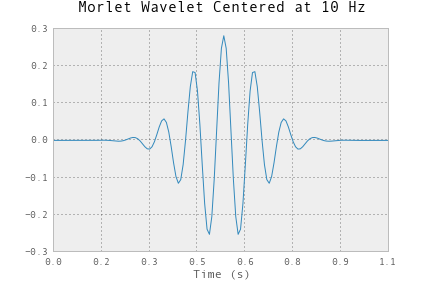
\includegraphics[width=4in]{morletwavelet}
\end{figure}


Wavelet decompositions are similar to Fourier Decompositions, but represent an EEG signal in a basis of functions known as “wavelets.”  One commonly used wavelet in EEG analysis is the Morlet wavelet.  It consists of a temporally-centered sine wave whose amplitude decays as a Gaussian with distance from its center.  Wavelets, although computationally expensive to calculate, provide the temporal resolution that Fourier analysis fails to capture.  

	In this experiment, we performed face/place classification using a Morlet wavelet basis.  We used wavelets spaced from 1 to 60 Hertz on a logarithmic scale.  The results of a wavelet decomposition of a single participant over a single trial are shown in figure \ref{wavelet_decomp}.  

\begin{figure}[t]
\centering
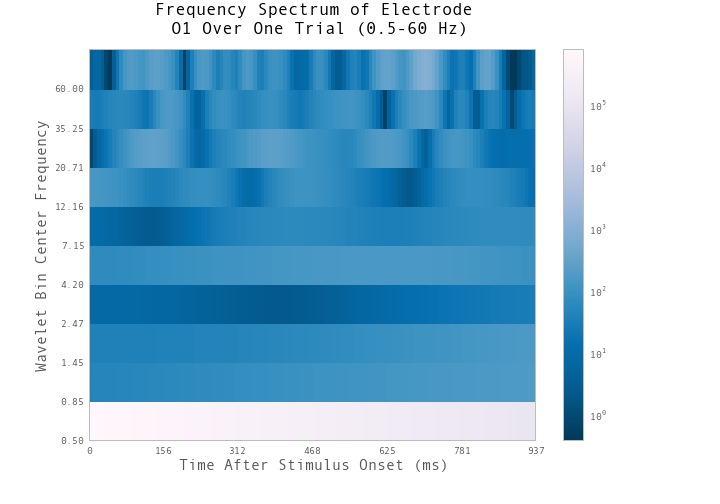
\includegraphics[width=6in]{wavelet_transform_O1_halfto60}
\caption{Wavelet decomposition of electrode O1\label{wavelet_decomp}}
\end{figure}

\begin{figure}[t]
\centering
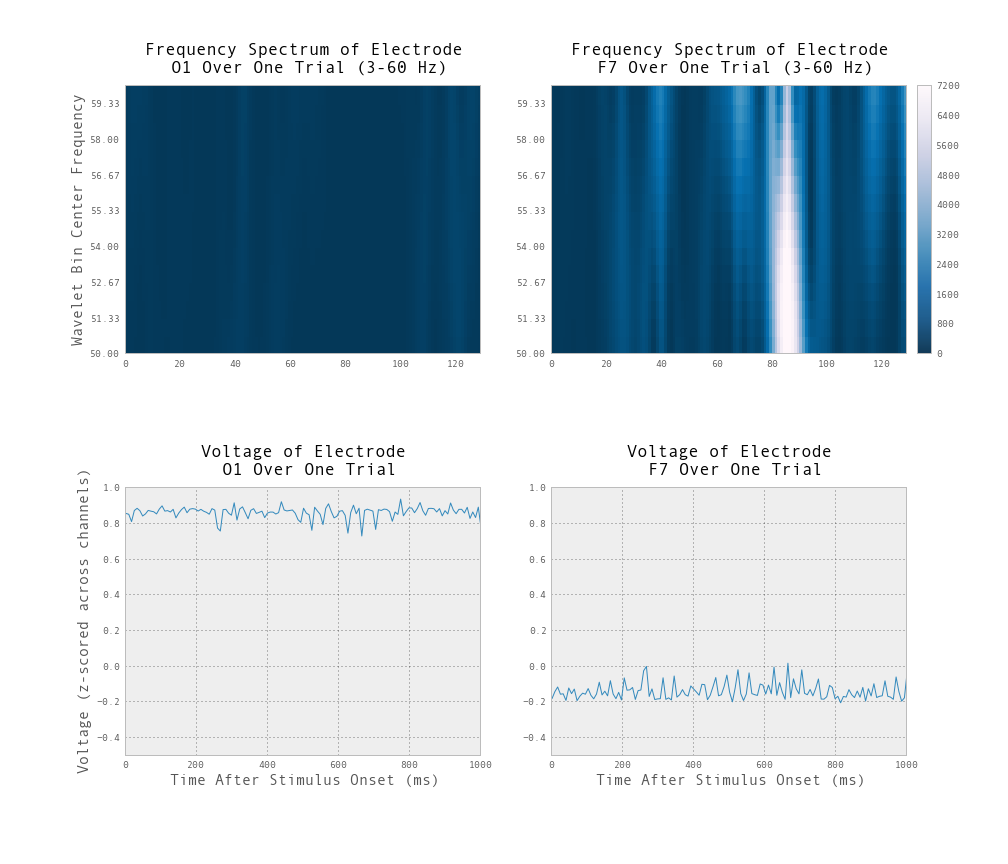
\includegraphics[width=5.5in]{eyebink_wavelets_compare}
\caption{Eyeblinks can be seen easily in frequency space for electrode F1}
\end{figure}

\subsubsection{Time Binning}
	In order to preserve timing information in EEG data classification, data in all analyses were time binned.  That is, values were calculated over all points in a time bin, and averaged over that time bin.  For example, we might analyze data by chunking it into 100 millisecond time bins, and train a unique classifier for all 
\subsubsection{Removing Baseline Signal}
	When a subject begins a trial, they experience a reaction to the shown stimulus which we posit decays over the course of the 1,000 millisecond trial.  In order to remove the "baseline" signal which represents the participant's EEG signal after stimulus response has decayed, we subtract the average voltage on all of the channels over the last 80 milliseconds of the preceding trial from the current trial.  Doing so slightly improved performance for time binned analysis.
	
\subsubsection{Dimensionality Reduction}
Principal Component Analysis or PCA is a dimensionality reduction technique that takes as input a data array and a number k, and returns a set of k vectors such that the first vector has the highest possible variance within the given data, the second vector has the second highest variance given the constraint that it is orthogonal to first vector, and so on.  From a different view, the PCA analysis on a dataset yields the eigenvectors of the covariance matrix of that data.

	Note: I'm using PCA because Jeremy said this worked the best for his data.  He used all components whose eigenvalues were above 1 (Kaiser 1960).

\subsection{Machine Learning Classifiers}
\subsubsection{Logistic Regression with Penalization}

A logistic regression is a simple linear model which takes as input n-dimensional training points and labels, and models the relationship between input vectors and labels as 	the outcome of Bernoulli trials ... {\bf tbd}

\subsubsection{Support Vector Machines}

\begin{figure}[t]
\centering
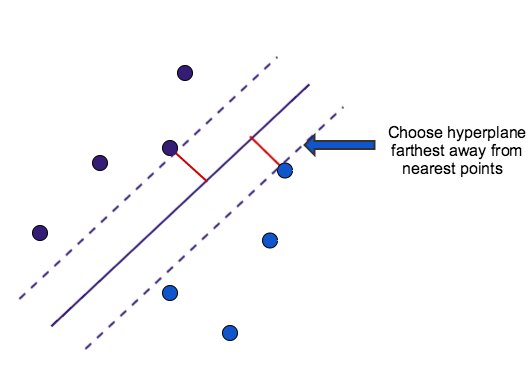
\includegraphics[width=4in]{svm}
\caption{Support Vector Machines find the a separating hyperplane between points in $X$ in $Y$ that maximizes the distance between the hyperplane and those points nearest to the hyperplane.}
\end{figure}

	Support Vector Machines (SVMs) are a commonly used ``off-the-shelf'' classifier for BCI applications.  In their most basic form, SVMs work as follows:  data are provided as a n-dimensional vectors, with each point labeled -1 or 1 (faces or places, in this case).  Let all training points that are labeled as faces be contained in the set $X$, and all points labeled as places fall in the set $Y$.  Then the SVM algorithm then finds an n-1 dimensional hyperplane $\mathbb{H} = \{x\in \mathbb{R}| A^Tx=b\}$ for some matrix $A$ and $b\in \mathbb{R}$, chosen such that the Euclidean distance between the points in $X$ and $Y$ closest to $\mathbb{H}$ is maximized.  In other words, the SVM algorithm finds:
		$$ \argmax_{A,b} \min_{z\in X\cup Y} d(H,z) $$,
		
		where $d(H,z)$ is the Euclidean distance between $H$ and $z$.
		
	As described above, an SVM divides data that is linearly separable.  However, a small modification can allow SVM's to quickly classify data that is not linearly separable.  SVM algorithms maximize the Euclidean distance between points and hyperplanes in a way that depends only on a calculation of dot products.  It is possible to map input feature vectors into arbitrarily high dimensional space using a variety of methods, changing the dot products of the vectors in the new space.  If the dot product of vectors in this new space is a simple function of the vectors in the lower dimensional space, the an SVM algorithm can use this dot product function, also known as a ``kernel trick'', to calculate a margin-maximizing hyperplane between points in this higher dimensional space.  Past BCI experiments have successfully used Gaussian and 	Radial Basis Function kernels to classify EEG data\cite{Lotte}.



\section{Results}

\begin{figure}[t]
\centerline{
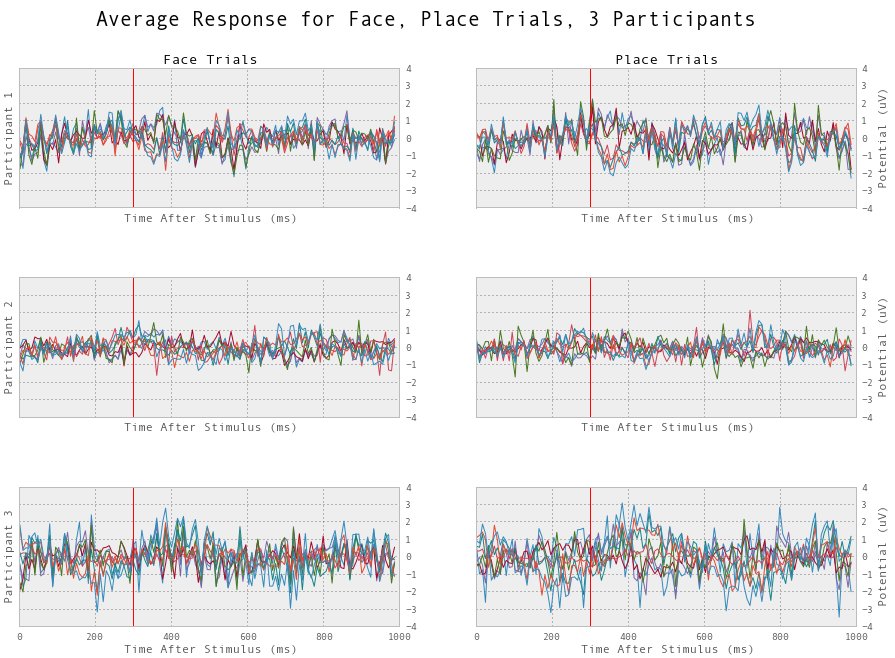
\includegraphics[width=6in]{3partsfaceplace}
}
\caption{Average EEG Signal Over Face/Place Trials for 3 Participants.  Channels F3, F4, FC5, P7, P8, O1 and O2 are shown) \label{3partsfaceplace}}
\end{figure}

We begin by visually inspecting the average voltages across all face/place trials of three participants, as shown in figure \ref{3partsfaceplace}.  These three participants were chosen because they showed the highest classifiability when analyzed in section \ref{timebin}.  The vertical red line denotes the time point 300 milliseconds after stimulus onset, which where the P300 EPR (as discussed below) occurs.  Visual inspection alone does not give an obvious explanation for the difference between these trials, but does show a faint 2-3 Hz signal in most cases.  This suggests that frequency analysis, especially focusing on the delta band (0-4 Hz), might prove fruitful.

\subsection{Simple Time Bin Analysis \label{timebin}}

In this experiment, we assume that a participant's mental response to a shown stimulus is time-locked.  Event-Related Potentials (ERPs), for example, are common EEG signals that occur as voltage changes at fixed times after a stimuli is shown.  Thus, we would like to analyze data in such a way that preserves temporal information about EEG signal.  Perhaps the simplest method of preserving time information is to analyze data in time bins.  In the analysis shown in figure \ref{nfoldsimple}, data from eleven participants was extracted at various offsets from the stimulus onset over various bin widths.  For each (stimulus offset, time bin) pair, a model was trained for each participant over this data.  In particular, the features of the model consisted of the average voltages over each of the fourteen channels, starting at time \textbf{stimulus-offset} and ending at time \textbf{stimulus-offset + binwidth}.  Features were then z-scored across channels, so that the resulting 14-dimensional feature vectors represented the relative magnitude of voltages of the channels relative to one another.  Thus a single feature vector was created for each trial, resulting in 50 features per block $\times$ 30 blocks per participant.  The labels for each of these features was the category (faces or places) the participant was instructed to attend to. For each participant and (\textbf{ stimulus-offset}, \textbf{binwidth}) pair, a Logistic Regression model with L2 penalization was trained and evaluated over 12 folds.  The data for each participant represented 30 minutes of viewing overlaid images of faces and places at 50/50 opacity.

\begin{figure}[t]
\centerline{
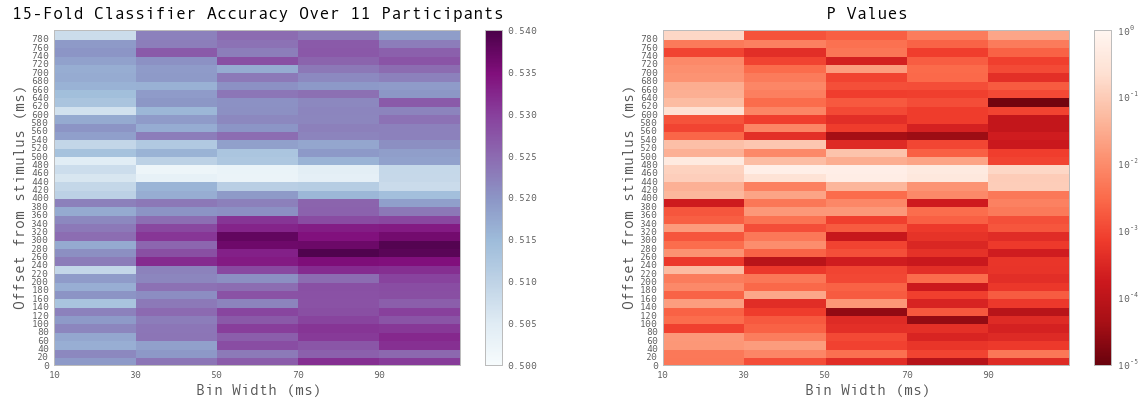
\includegraphics[width=7in]{gridsearch_logreg_simple}
}
\caption{12-Fold classifier accuracy over various bin widths and offsets after stimuli, 11 participants.\label{nfoldsimple}}
\end{figure}

The results of this analysis as shown in Figure \ref{nfoldsimple} indicate that, for the eleven participants sampled, classification accuracy was highest at 280 milliseconds after stimulus onset with a bin width of 90 milliseconds.  With these parameters, classification accuracy is 0.54 with a standard deviation of 0.06 across participants (p value $10^{-4}$).  The location of this increase in accuracy suggests that the classifier is perhaps capturing the P300 EPR, which is a positive deflection in voltage that begins at roughly 250 to 300 milliseconds after the participant is shown an outlier or ``oddball'' stimuli\cite{p300}.  In this experiment, we would expect the P300 to be most prominent during lure trials.  Figure \ref{luresvsnonlures300} shows the average voltages over trials of a single participant, seperated into lure trials and non lure trials for faces and places respectively.  The channels displayed are those found to be most effective for detecting the P300 signal on the Emotiv according to \cite{Ekanayake}.  The P300 is not clearly visible in Figure \ref{luresvsnonlures300}, although visual inspection of several participants shows to that voltages are of higher magnitude in general for lure trials as opposed to non-lure trials.  

     
\begin{figure}[t]
\centerline{
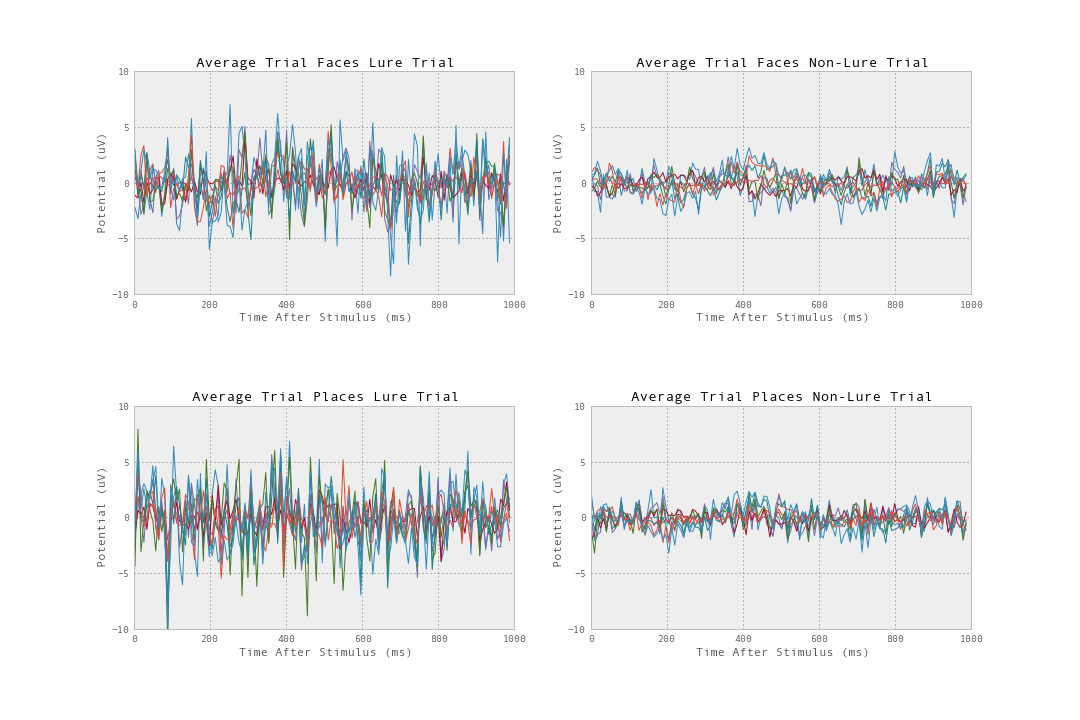
\includegraphics[width=7in]{lurevsnonlurep300}
}
\caption{12-Fold classifier accuracy over various bin widths and offsets after stimuli using wavelet decomposition as features, 12 participants.\label{luresvsnonlures300}}
\end{figure}

\subsection{Wavelet Time Bin Analysis}

A similar analyses as in section \ref{timebin} was conducted, using time bins and Logistic Regression to classify data.  In this analysis, however, EEG data was processed into a series of wavelets before being broken into time bins for classification.  In particular, each channel was decomposed into 10 frequency bands logarithmically spaced from 0.5 Hz to 60 Hz.  The resulting feature vector was 14 $\times$ 10 dimensional (10 frequencies for each channel), representing the power of each channel in each of 10 frequency ranges averaged over a time bin.  Figure \ref{wavelet_gridsearch} shows that this wavelet decomposition performed very near chance over all time bins.

\subsection{Hilbert Transform Analysis}  

I will try this time permitting (jeremy's suggestion).

\begin{figure}[t]
\centerline{
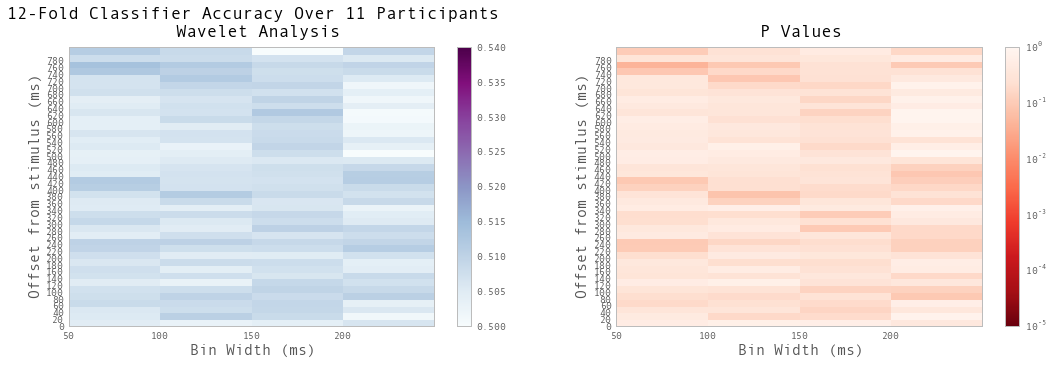
\includegraphics[width=7in]{wavelet_gridsearch.png}
}
\caption{12-Fold classifier accuracy over various bin widths and offsets after stimuli using wavelet decomposition as features, 11 participants.\label{wavelet_gridsearch}}
\end{figure}


\subsection{Component Analysis}

Time permitting, I may explore classification accuracy using PCA components (jeremey suggestion).

\subsection{Classifiers}

This section will include the accuracy of different classifiers on the data set, including SVM, KNNR, Logistic Regression with different penalization methods (jeremey suggestion), etc.  I've looked at these before but just haven't plotted the results.  They all perform roughly the same.

\subsection{Classification Accuracy versus Participant Accuracy}

A major hypothesis of this experiment was the notion that classifier accuracy is correlated with a subject's ability to focus intently on faces while ignoring places, or the reverse.  Consider, for example, an SVM that divides face/place data points as shown below.  We predict that a participant who can concentrate well on the face/place task produces EEG readings that are separable by some learning algorithm, in this case an SVM hyperplane.  We further predict that when a participant is concentrating poorly, his/her EEG readings lie closer to the hyperplane i.e. face/place concentration boundary than when he/she is focusing intently on one category or the other, due to ``noise'' from concentration on the competing category. 

To test our first hypothesis, we consider how well a participant's classifier accuracy predicts that participant's performance on responding to lure trials.  For each participant, we train a Logistic Regression model on time binned data of 100 milliseconds starting 280 milliseconds after stimulus onset.  We evaluate 12-fold classifier accuracy for each participant.  We then compare this measurement to the participant's percent correct responses on lure trials.  If our hypothesis is correct, the participants whose classifiers were more accurate were less distracted, and thus would have performed better at the task.  We evaluate a participant's performance on the task as the ratio of correct rejections on lure trials to the total number of lure trials.  It is not unusual in this task for a participant to score around 0.5, since the lure trials occur so much more infrequently than the non-lure trials that participants often accidentally ``false alarm'' on the lure trials due to momentum.  The results of this analysis are given in figure \ref{responsevsclass}, and show that with the current data, there did not appear to be a strong relationship between classifier accuracy and participant lure response accuracy.

\begin{figure}[t]
\centerline{
	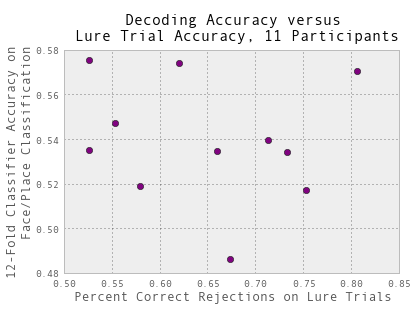
\includegraphics[width=4.5in]{response_acc_vs_class_acc}
}
\caption{15-fold classifier accuracy over various bin widths and offsets after stimuli.\label{responsevsclass}}
\end{figure}

In addition to the above analysis, within a single participant, we would like to know whether a participant's brain was ``more classifiable'' when he/she performed well on lure trials than when he/she made an incorrect response before lure trials.  A logistic regression model provides a measure of ``confidence'' for each of its predictions, which is the model's estimate of the probability of the given sample point of belonging to each of two categories.  We can think of the difference between these two probabilities, then, as representing how far the given data is from the model's decision boundary.  We would like to know if a particular participant's EEG readings were closer to this decision boundary before the participant made a mistake (false alarm) than before the participant responded to the lures correctly (correct rejection).  We plot the average difference in category probabilities before correct rejections and false alarms over 11 participants in figure \ref{falsealarmcorrectreject}, over the four trials preceding a lure trial and the lure trial itself.  

\begin{figure}[t]
\centerline{
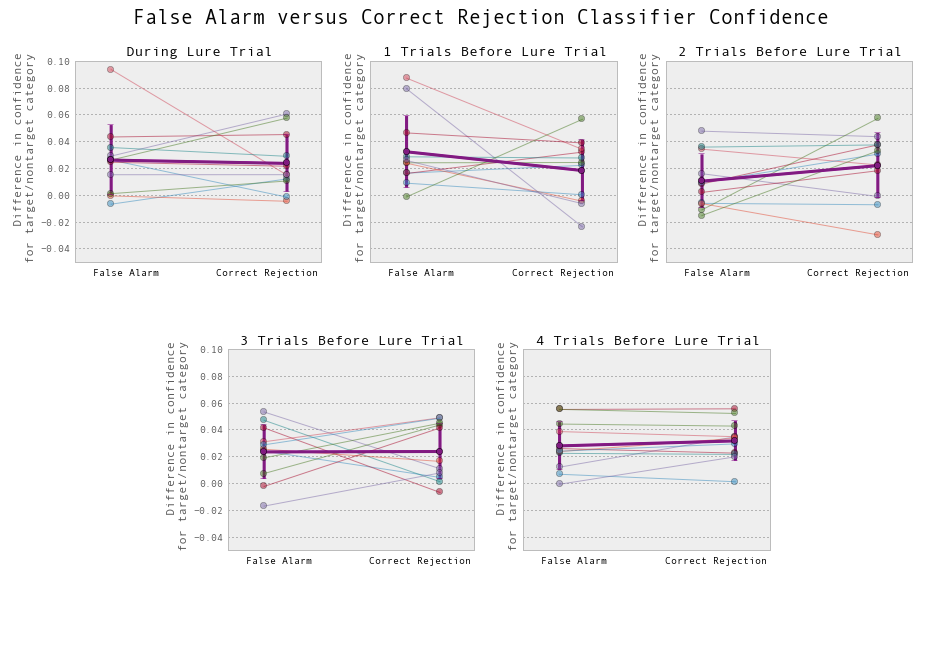
\includegraphics[width=6in]{trialsbeforelureacc}
}
\caption{Classifier accuracy before false alarms versus correct rejectinos.\label{falsealarmcorrectreject}}
\end{figure}

This results did not show a strong relationship between classifier confidence between false alarm and correct rejection trials.

\subsection{Realtime Feedback}

A core goal of this experiment was to study how well humans can learn to control their sustained attention using feedback generated on the basis of the content of their thoughts.  In this experiment, training was achieved by altering the opacity of the target category image on the basis of the participant's level of concentration on that category.  Because of its simplicity, we chose to provide participants with feedback calculated on the basis of a logistic regression classifier with L2 regularization, calculated on a z-scored, 100 ms time bin that began 100 ms after stimulus onset.  These parameters were chosen based on a small sample set of early participants; a more accurate way to have chosen parameters would have been to choose the best time bin and offset for a participant on-the-fly, but this would have introduced programming complexity.  The code for the calculation of this feedback can be found in the Appendix.  The exact face/place image ratio for the feedback was calculated by looking at the classifier confidence calculated for the trial preceding the current trial.  This classifier confidence fell between a range of 1 for perfect concentration on the target category, and -1 for perfect concentration on the distractor category.  Because difference in classifier confidence was usually quite small (< 0.1), the difference was amplified via the function shown in Figure \ref{sigmoid}.  The target category image opacity was allowed to reach 0.9, but was never allowed to fall below 0.3.  

\begin{figure}[t]
\centering
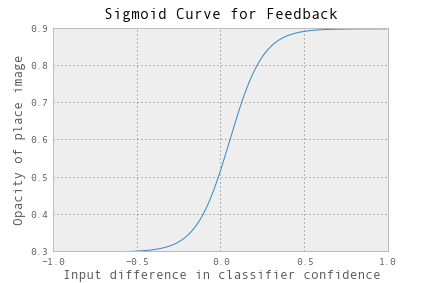
\includegraphics[width=4.5in]{sigmoidcurve}
\caption{Sigmoid curve maps classifier confidence differences to image opacity values, ensuring that opacity is scaled appropriately to the range of classifier confidence read by the Emotiv\label{sigmoid}}
\end{figure}

Figure \{avgfeedbacktrial} shows the average feedback over trials a single participant received over the course of the experiment.  
\begin{figure}[t]
\centering
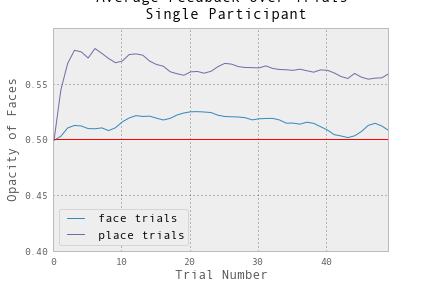
\includegraphics[width=4.5in]{average_feedback_trial}
\caption{Average feedback received by one participant over all trials.\label{avgfeedbacktrial}}
\end{figure}
  
\bibliography{bib}{}
\bibliographystyle{plain}


\end{document}
